\documentclass[12pt]{article}

\usepackage{blindtext} % Package to generate dummy text throughout this template 

\usepackage[utf8]{inputenc}
\usepackage{amsmath, amssymb}
\usepackage{algorithm}
\usepackage{algpseudocode}
%\usepackage{times} % Use the Times font
%\usepackage[T1]{fontenc}
\linespread{1.25}
\usepackage[margin = 1in]{geometry}
\usepackage{microtype} % Slightly tweak font spacing for aesthetics
\usepackage[english]{babel} % Language hyphenation and typographical rules
\usepackage{tikz}
\usepackage[hidelinks]{hyperref}
\usepackage{url}
\usepackage{graphicx}
\usepackage{float}
\usepackage{wrapfig}

\setlength{\parindent}{2em}
%\setlength{\parskip}{1.5em}
\graphicspath{ {images/} }

\newcommand{\vect}[1]{\mathbf{#1}}  % vector
\newcommand{\matr}[1]{\mathbf{#1}}  % matrix
\newcommand{\tens}[1]{\mathbf{#1}}  % tensor
\newcommand{\mean}[1]{\overline{#1}}    % mean overline

\begin{document}
    \tableofcontents
    \listoftables
    \listoffigures
    \section{Introduction} \label{sec:introduction}
    Optimizing predictive models on datasets that are obtained from citizen-science projects can be computationally expensive as these datasets grow in size with time. Consequently, models based on multiple-layered Neural Networks, Integer Programming and other optimization routines can prove increasingly difficult as the number of parameters increase, despite using the faster Central Processing Units (CPUs) in the market. Incidentally, it becomes difficult for citizen-science projects to scale if the organizers use CPUs to run optimization models. However, Graphical Processing Units (GPUs), which offer multiple cores to parallelize computation, can outperform CPUs in computing such predictive models if these models heavily rely on large-scale matrix multiplications. By using GPUs over CPUs to accelerate computation on a citizen-science project, we have been able to achieve better optimization in less time, enabling the project to scale.\\
    
    Part of the eBird project, which aims to ``maximize the utility and accessibility of the vast numbers of bird observations made each year by recreational and professional bird watchers'', Avicaching is a incentive-driven game trying to homogenize the spatial distribution of citizens' observations [cite website]. One such predictive model is Avicaching \cite{Xue2016Avi1} in the eBird platform [cite], which aims to  [cite website]. Since the eBird dataset is heterogeneous geographically, Avicaching tries to homogenize future observations by providing observer-citizens incentives to visit under-sampled locations \cite{Xue2016Avi1}. Therefore, the Avicaching game can be modeled as two separate problems - identifying parameters of citizens' behavior on a specific set of rewards (incentives), and pooling rewards from a budget to locations such that the citizens' predicted behavior is homogeneous \cite{Xue2016Avi2}.
    
    \subsection{Identification Problem} \label{sec:iden_problem}
    This subroutine will learn parameters of the change in citizens' behavior due to rewards. Specifically, given datasets $\vect{y_t}$ and $\vect{x_t}$ of citizens' visit densities with and without the rewards $\vect{r_t}$, we want to find weights $\matr{w_1}$ and $\matr{w_2}$ that caused the change from $\vect{x_t}$ to $\vect{y_t}$, factoring in possible influence due to environmental factors $\matr{f}$ and distances between locations $\matr{d}$. Although the original model proposed to learn a single set of weights $\matr{w}$, our proposed model considers two sets of weights $\matr{w_1}$ and $\matr{w_2}$ as it may theoretically result into higher accuracy and lower loss. Mathematically, our model can be formulated as:
    \begin{equation} \label{eq:iden_problem}
    \begin{aligned}
    & \underset{\matr{w}}{\text{minimize}}
    & & Z_I(\matr{w}) = \sum_{t} (u_t(\vect{y_t} - \matr{P}(\matr{f}, \vect{r_t}; \matr{w_1}, \matr{w_2})\vect{x_t}))^{2}
    \end{aligned}
    \end{equation}
    where $u_t$ is the total number of submissions at time $t$ for a given citizen and elements $p_{u, v}$ of $P$ are given as:
    \begin{equation} \label{eq:puv_equation}
    p_{u, v} = \frac{\exp(\matr{w_2} \cdot \text{reLU} (\matr{w_1} \cdot [d_{u, v}, \vect{f_{u, v}}, r_{u}]))}{\sum_{u'} \exp(\matr{w_2} \cdot \text{reLU} (\matr{w_1} \cdot [d_{u', v}, \vect{f_{u', v}}, r_{u'}]))} = \frac{\exp(\Gamma_{u, v})}{\sum_{u'}\exp(\Gamma_{u', v})} = \text{softmax}(\Gamma_{u, v})
    \end{equation}
    In the expression for $p_{u,v}$ (equation \ref{eq:puv_equation}), softmax is the function: softmax$(z_i) = \frac{\exp(z_i)}{\sum_{i}\exp(z_i)}$ and the reLU$(\cdot)$ function is a rectified Linear Unit defined as: reLU$(z) = \text{max}(0, z)$.
    
    \subsection{Pricing Problem} \label{sec:pricing_problem}
    The Pricing subroutine will attempt to allocate rewards to all locations such that the predicted behavior is least heterogeneous, given the learned parameters from Section \ref{sec:iden_problem}. This optimization problem can be written as:
    \begin{equation} \label{eq:pricing_problem}
    \begin{aligned}
    & \underset{\vect{r}}{\text{minimize}}
    & & Z_P(\vect{r}) = \frac{1}{n}\lVert \vect{y} - \mean{\vect{y}} \rVert\\
    & \text{subject to}
    & & \vect{y} = \matr{P}(\matr{f}, \vect{r}; \matr{w_1}, \matr{w_2}) \, \vect{x}\\
    &&& \sum_{i} r_i \leq \mathcal{R}\\
    &&& r_i \geq 0
    \end{aligned}
    \end{equation}
    where $\mathcal{R}$ is total reward budget and $\matr{P}$ is defined as in Equation \ref{eq:puv_equation}.
    
    \subsection{Computation Using GPUs} \label{sec:comp_using_GPUs}
    
    \section{Problem Formulation}
    Since NVIDIA General Purpose GPUs enable faster computation on matrices, accelerated through CUDA and cuDNN, both the Identification Problem (Section \ref{sec:iden_problem}) and Pricing Problem (Section \ref{sec:pricing_problem}) were formulated as 2-layer Neural Networks using the PyTorch platform.
    
    \subsection{Design for Identification Problem}
    
    The Identification Problem (Section \ref{sec:iden_problem}) can be modeled as a typical 2-layered Neural Network, which learns the weights through multiple iterations of back-propagating the loss value $Z_I(\matr{w})$ (equation \ref{eq:iden_problem}) using gradient descent.
    
    \subsubsection{Structure of Input Dataset}
    \begin{figure}[h]
        \centering
        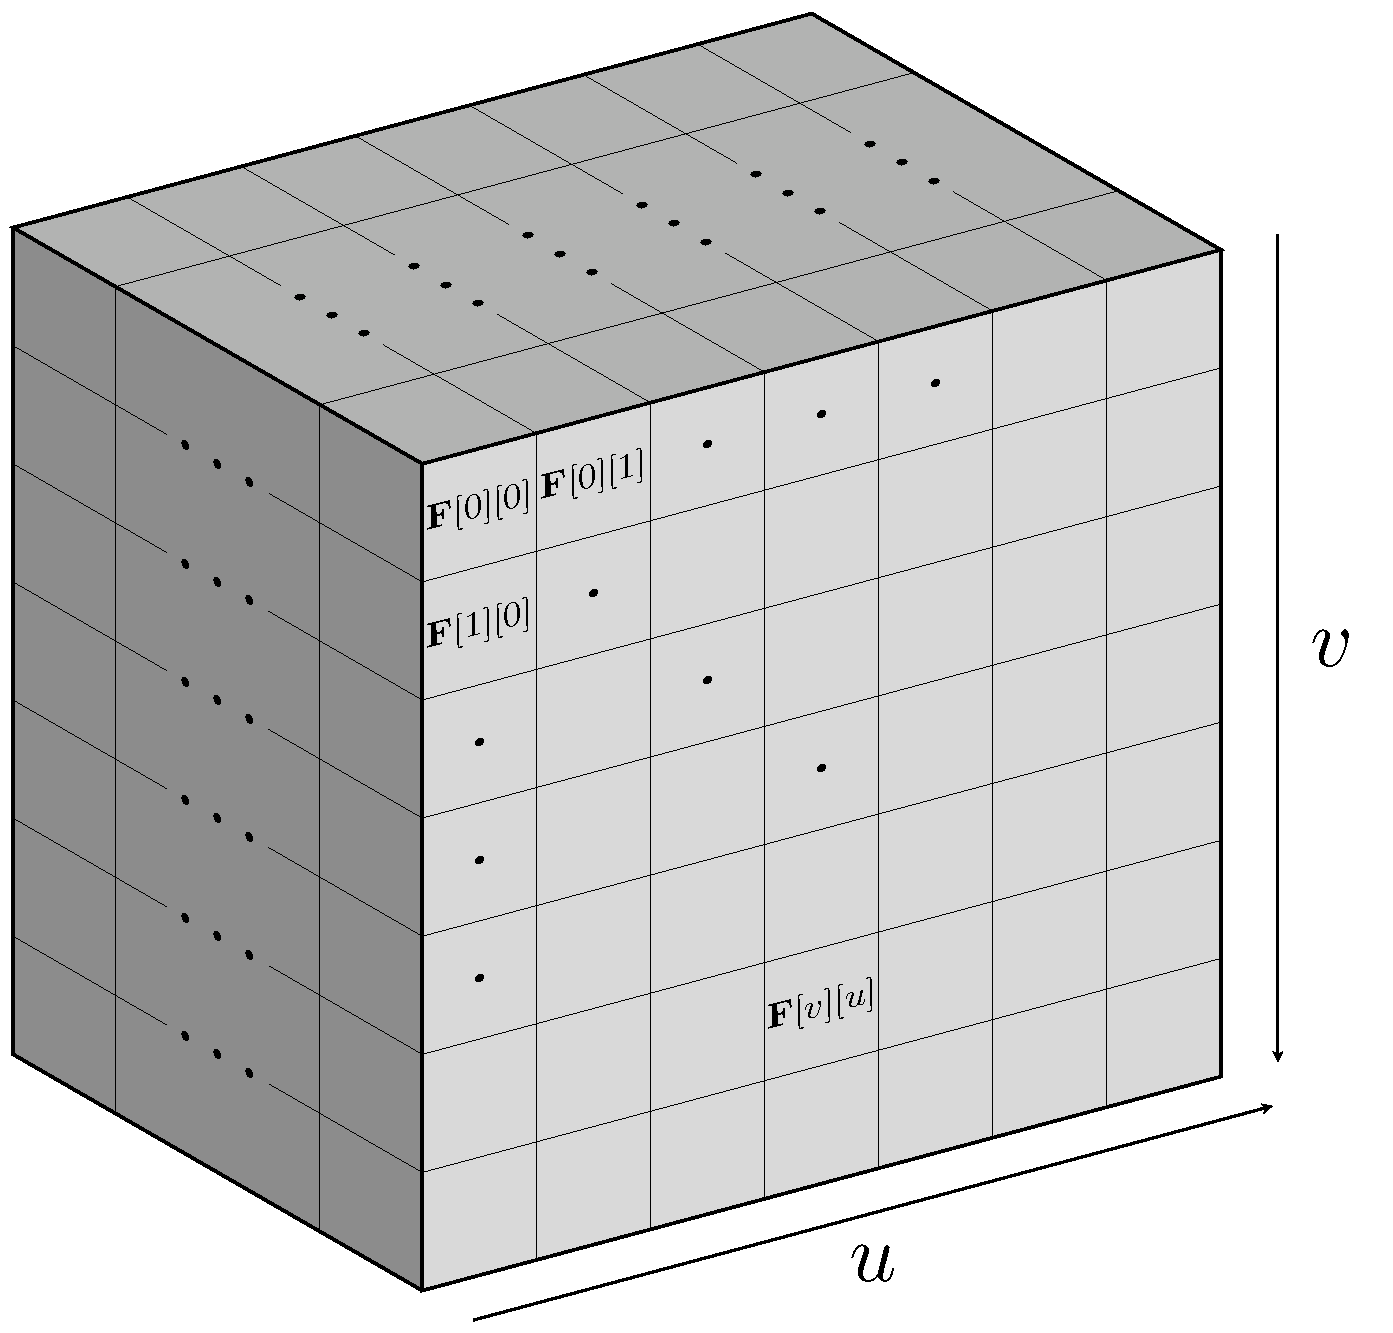
\includegraphics[width=.4\textwidth]{weights_input_dataset}
        \caption{A Tensor representing the Input Dataset}
        \label{fig:A Tensor representing the Input Dataset}
    \end{figure}
    
    \begin{wrapfigure}{r}{0.4\textwidth}
        \centering
        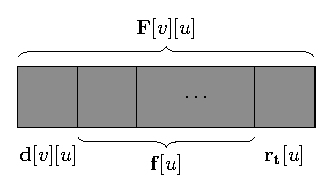
\includegraphics[width=0.3\textwidth]{zoomup_Fuv}
        \caption{Contents of $\vect{F}_{vu}$}
        \label{fig:Contents of Fvu}
    \end{wrapfigure}
    The input dataset comprising of environmental features $\vect{f}$ and given rewards $\vect{r_t}$ must be combined into a tensor (figure \ref{fig:A Tensor representing the Input Dataset}) that can be readily operated on by NVIDIA GPUs. Another advantage of building the dataset as discussed comes with the PyTorch library, which provides convenient handling of tensors residing on CPUs as well as GPUs. Algorithm \ref{alg:Constructing the Input Dataset} describes the steps to construct this dataset.
    
    \begin{algorithm}
        \caption{Constructing the Input Dataset} \label{alg:Constructing the Input Dataset}
        \begin{algorithmic}[1]
            \State $\matr{d} \gets \Call{Normalize}{\matr{d}}$\Comment{$\matr{d}[u][v]$ is the distance between locations $u$ and $v$}
            \State $\vect{f} \gets \Call{Normalize}{\mathbf{f}, axis = 0}$\Comment{$\mathbf{f}[u]$ is a vector of env. features at location $u$}
            \State $\vect{r_t} \gets \Call{Normalize}{\vect{r_t}, axis = 0}$\Comment{$\vect{r_t}[u]$ is the reward at location $u$}
            \For{$v = 1, 2, \dots J$}
                \For{$u = 1, 2, \dots J$}
                    \State $\tens{F}[v][u] \gets [\matr{d}[v][u], \vect{f}[u], \vect{r_t}[u]]$ \Comment{Figure \ref{fig:Contents of Fvu}}
                \EndFor
            \EndFor
        \end{algorithmic}
    \end{algorithm}
       
    \subsubsection{Algorithm for Identification Problem}
    For learning the weights $\matr{w}$ in equation \ref{eq:iden_problem}, a Neural Network was built using the PyTorch library, which minimized the loss function using gradient descent routines. Figure \ref{fig:Neural Network designed for Identification Problem} illustrates the framework of the network used, calculating the vector $\vect{p_v}$. This network was fed in with data from different locations $v$, resulting into the matrix $\matr{P}$, which was then used to calculate the loss.
    \begin{figure}[H]
        \centering
        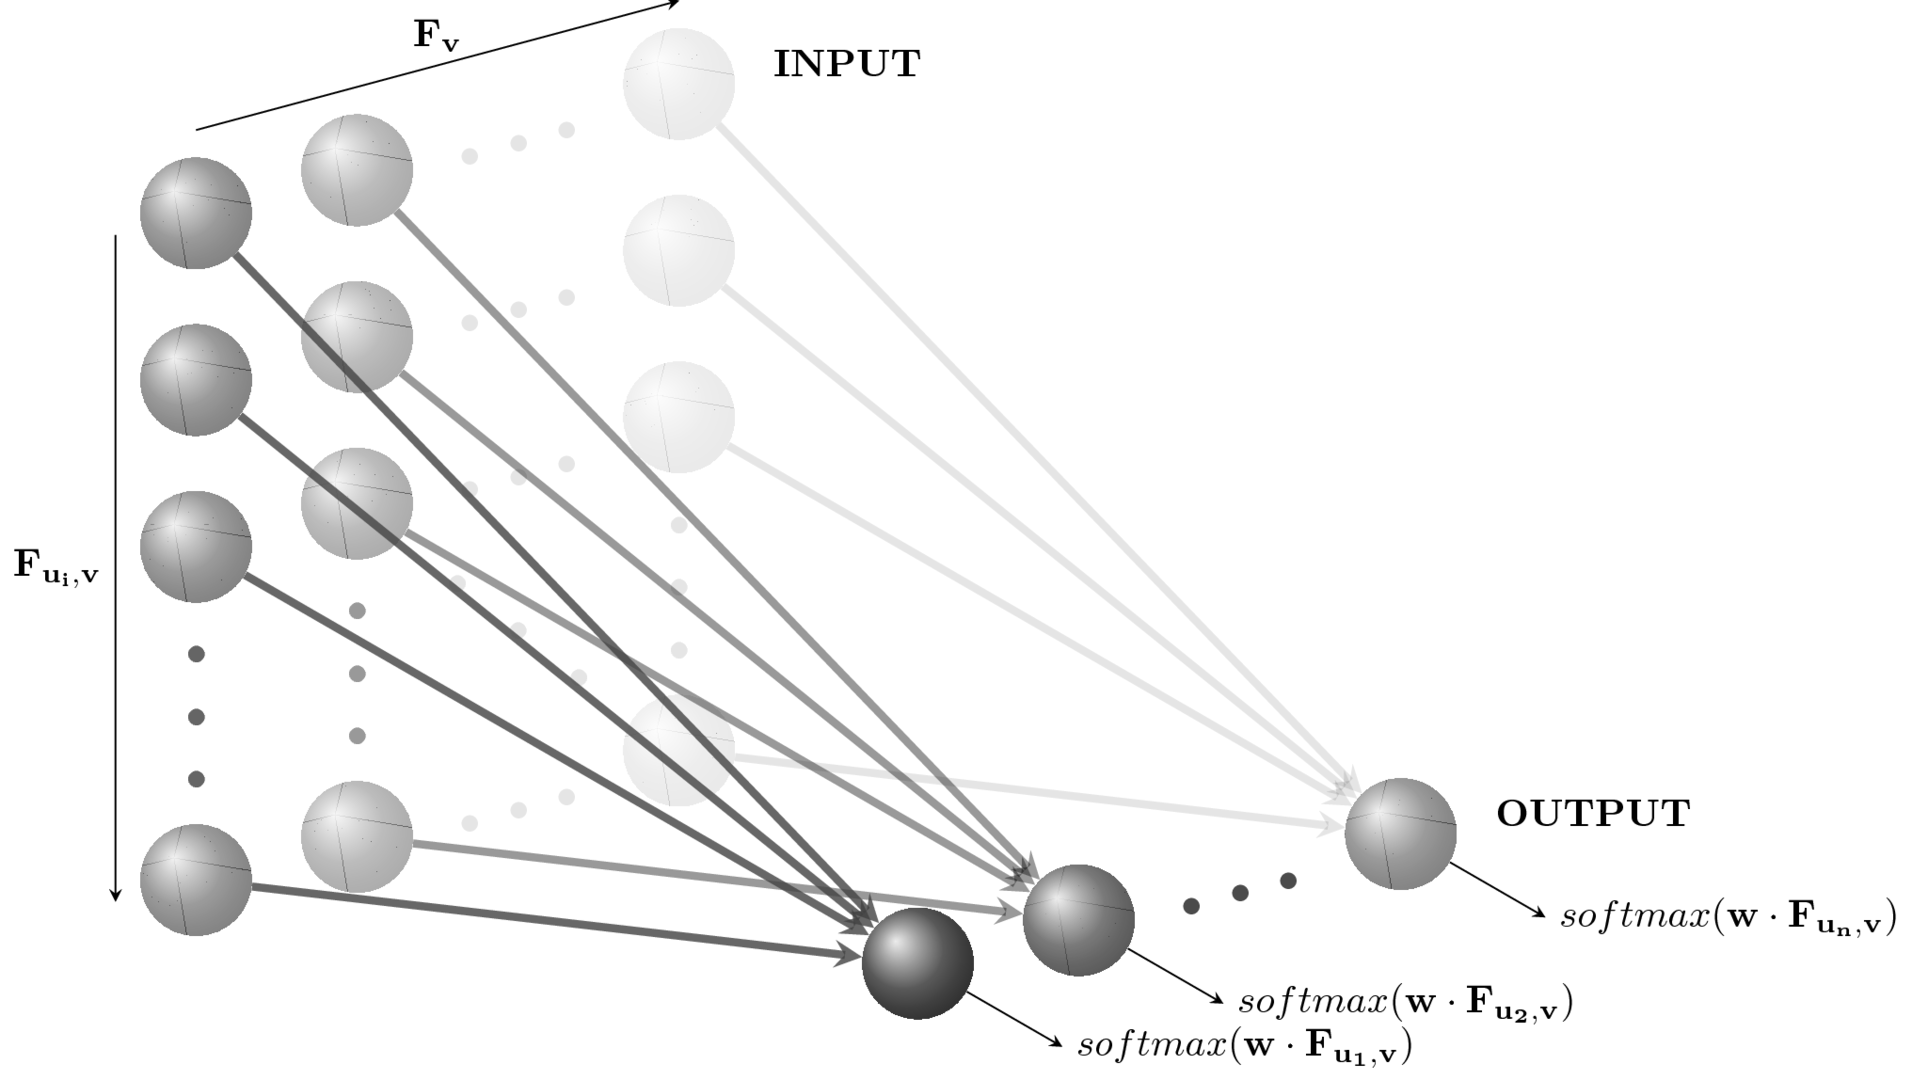
\includegraphics[width=\textwidth]{weights_net}
        \caption{Neural Network designed for Identification Problem}
        \label{fig:Neural Network designed for Identification Problem}
    \end{figure}
    An algorithm for the optimization problem is described in Algorithm \ref{alg:Optimizing for the Identification Problem}.
    \begin{algorithm}
        \caption{Optimizing for the Identification Problem} \label{alg:Optimizing for the Identification Problem}
        \begin{algorithmic}[1]
            \State $a \gets b$
        \end{algorithmic}
    \end{algorithm}
    \section{Experiments}
    
    \section{Results}
    \section{Conclusion}
    
    \blindtext
    \bibliographystyle{ieeetr}
    \bibliography{avicaching}
\end{document}